% LLM Architecture: How All Components Work Together for Next-Token Prediction
% Compile with: pdflatex llm_architecture_nexttoken.tex

\documentclass[tikz,border=10pt]{standalone}
\usepackage{tikz}
\usetikzlibrary{arrows.meta,positioning,shapes.geometric,fit,backgrounds,decorations.pathreplacing}

\definecolor{embedcolor}{RGB}{100,150,200}
\definecolor{layercolor}{RGB}{150,180,100}
\definecolor{outputcolor}{RGB}{220,120,100}
\definecolor{tokencolor}{RGB}{180,140,200}
\definecolor{gradcolor}{RGB}{255,200,100}

\begin{document}

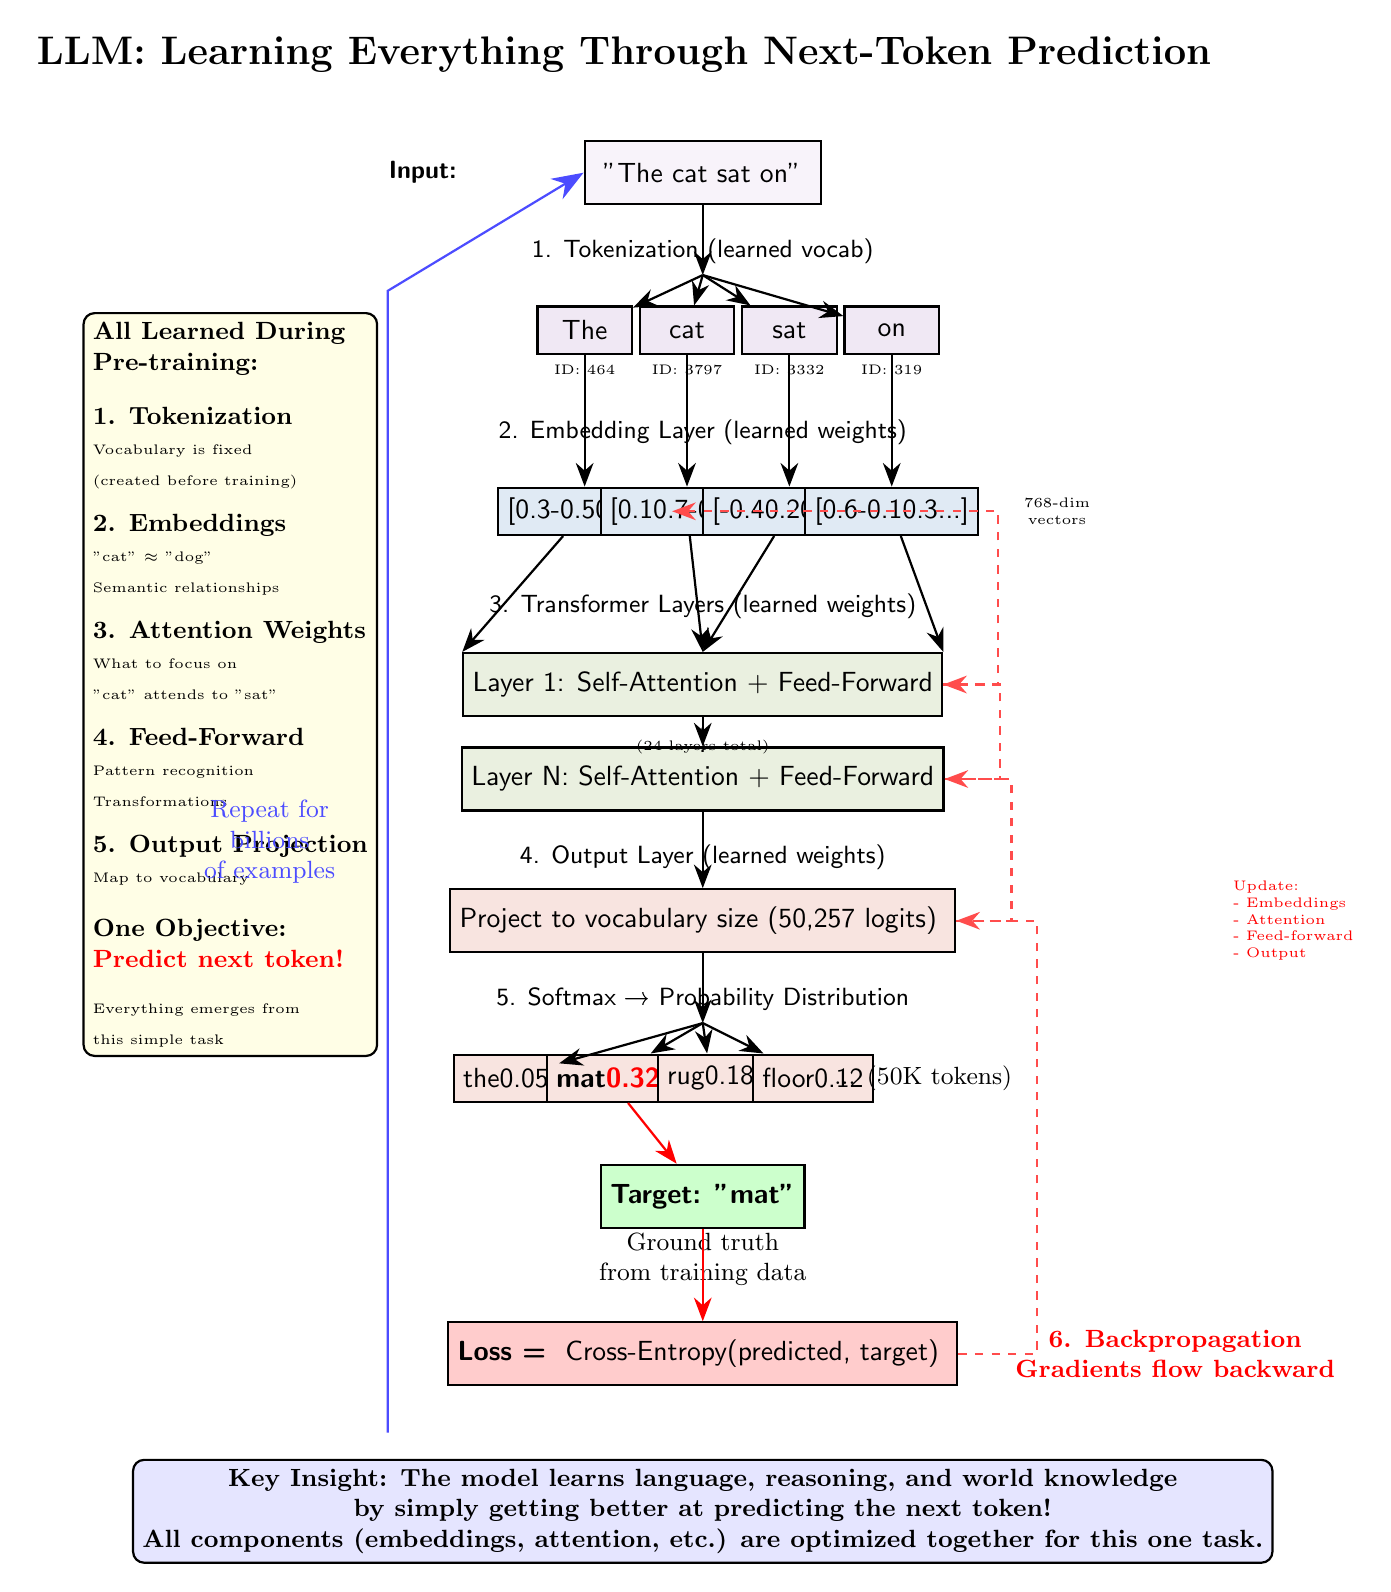
\begin{tikzpicture}[
    font=\sffamily,
    node distance=1.5cm,
    box/.style={rectangle, draw, thick, minimum width=3cm, minimum height=0.8cm, align=center},
    tokenbox/.style={rectangle, draw, thick, fill=tokencolor!20, minimum width=1.2cm, minimum height=0.6cm},
    embedbox/.style={rectangle, draw, thick, fill=embedcolor!20, minimum width=1.2cm, minimum height=0.6cm},
    layerbox/.style={rectangle, draw, thick, fill=layercolor!20, minimum width=3cm, minimum height=0.8cm},
    outputbox/.style={rectangle, draw, thick, fill=outputcolor!20, minimum width=1.2cm, minimum height=0.6cm},
    arrow/.style={-{Stealth[length=3mm]}, thick},
    backarrow/.style={-{Stealth[length=3mm]}, thick, dashed, red!70},
    label/.style={font=\small\sffamily}
]

% Title
\node[font=\Large\bfseries] at (0,11) {LLM: Learning Everything Through Next-Token Prediction};

% Input text
\node[label, anchor=east] at (-2,9.5) {\textbf{Input:}};
\node[box, fill=tokencolor!10] (text) at (1,9.5) {"The cat sat on"};

% Tokenization
\node[label] at (1,8.5) {1. Tokenization (learned vocab)};
\node[tokenbox] (t1) at (-0.5,7.5) {The};
\node[tokenbox] (t2) at (0.8,7.5) {cat};
\node[tokenbox] (t3) at (2.1,7.5) {sat};
\node[tokenbox] (t4) at (3.4,7.5) {on};

\draw[arrow] (text) -- (1,8.2);
\draw[arrow] (1,8.2) -- (t1);
\draw[arrow] (1,8.2) -- (t2);
\draw[arrow] (1,8.2) -- (t3);
\draw[arrow] (1,8.2) -- (t4);

% Token IDs
\node[label, font=\tiny] at (-0.5,7.0) {ID: 464};
\node[label, font=\tiny] at (0.8,7.0) {ID: 3797};
\node[label, font=\tiny] at (2.1,7.0) {ID: 3332};
\node[label, font=\tiny] at (3.4,7.0) {ID: 319};

% Embeddings
\node[label] at (1,6.2) {2. Embedding Layer (learned weights)};
\node[embedbox] (e1) at (-0.5,5.2) {[0.3\\-0.5\\0.8\\...]};
\node[embedbox] (e2) at (0.8,5.2) {[0.1\\0.7\\-0.2\\...]};
\node[embedbox] (e3) at (2.1,5.2) {[-0.4\\0.2\\0.9\\...]};
\node[embedbox] (e4) at (3.4,5.2) {[0.6\\-0.1\\0.3\\...]};

\draw[arrow] (t1) -- (e1);
\draw[arrow] (t2) -- (e2);
\draw[arrow] (t3) -- (e3);
\draw[arrow] (t4) -- (e4);

\node[label, font=\tiny, align=center] at (5.5,5.2) {768-dim\\vectors};

% Transformer Layers
\node[label] at (1,4.0) {3. Transformer Layers (learned weights)};

% Layer 1
\node[layerbox, minimum width=5.5cm] (layer1) at (1,3.0) {
    Layer 1: Self-Attention + Feed-Forward
};

% Layer N
\node[layerbox, minimum width=5.5cm] (layerN) at (1,1.8) {
    Layer N: Self-Attention + Feed-Forward
};

% Dots between layers
\node at (1,2.4) {\vdots};
\node[label, font=\tiny] at (1,2.2) {(24 layers total)};

\draw[arrow] (e1) -- (layer1.north west);
\draw[arrow] (e2) -- (layer1.north);
\draw[arrow] (e3) -- (layer1.north);
\draw[arrow] (e4) -- (layer1.north east);

\draw[arrow] (layer1) -- (layerN);

% Output Layer
\node[label] at (1,0.8) {4. Output Layer (learned weights)};
\node[box, fill=outputcolor!20, minimum width=5.5cm] (output) at (1,0.0) {
    Project to vocabulary size (50,257 logits)
};

\draw[arrow] (layerN) -- (output);

% Predictions
\node[label] at (1,-1.0) {5. Softmax → Probability Distribution};
\node[outputbox] (p1) at (-1.5,-2.0) {the\\0.05};
\node[outputbox] (p2) at (-0.2,-2.0) {\textbf{mat}\\{\color{red}\textbf{0.32}}};
\node[outputbox] (p3) at (1.1,-2.0) {rug\\0.18};
\node[outputbox] (p4) at (2.4,-2.0) {floor\\0.12};
\node[label, font=\small] at (3.8,-2.0) {... (50K tokens)};

\draw[arrow] (output) -- (1,-1.3);
\draw[arrow] (1,-1.3) -- (p1);
\draw[arrow] (1,-1.3) -- (p2);
\draw[arrow] (1,-1.3) -- (p3);
\draw[arrow] (1,-1.3) -- (p4);

% Training: Next token
\node[box, fill=green!20, minimum width=2cm] (target) at (1,-3.5) {\textbf{Target: "mat"}};
\node[label, align=center, font=\small] at (1,-4.3) {Ground truth\\from training data};

% Loss
\node[box, fill=red!20, minimum width=4cm] (loss) at (1,-5.5) {
    \textbf{Loss = } Cross-Entropy(predicted, target)
};

\draw[arrow, thick, red] (p2) -- (target);
\draw[arrow, thick, red] (target) -- (loss);

% Backpropagation
\node[label, align=center, font=\small\bfseries, text=red] at (7,-5.5) {
    6. Backpropagation\\Gradients flow backward
};

% Gradient arrows (backward)
\draw[backarrow] (loss.east) -- ++(1,0) |- (output.east);
\draw[backarrow] (output.east) -- ++(0.7,0) |- (layerN.east);
\draw[backarrow] (layerN.east) -- ++(0.7,0) |- (layer1.east);
\draw[backarrow] (layer1.east) -- ++(0.7,0) |- (e1.east);

% Annotations
\node[label, font=\tiny, align=left, text=red] at (8.5,0) {
    Update:\\- Embeddings\\- Attention\\- Feed-forward\\- Output
};

% Side panel: What's learned
\begin{scope}[on background layer]
\node[draw, thick, rounded corners, fill=yellow!10, align=left, font=\small, minimum width=3.5cm, minimum height=8cm] at (-5,3) {
    \textbf{All Learned During}\\
    \textbf{Pre-training:}\\[0.3cm]

    \textbf{1. Tokenization}\\
    {\tiny Vocabulary is fixed}\\
    {\tiny (created before training)}\\[0.2cm]

    \textbf{2. Embeddings}\\
    {\tiny "cat" $\approx$ "dog"}\\
    {\tiny Semantic relationships}\\[0.2cm]

    \textbf{3. Attention Weights}\\
    {\tiny What to focus on}\\
    {\tiny "cat" attends to "sat"}\\[0.2cm]

    \textbf{4. Feed-Forward}\\
    {\tiny Pattern recognition}\\
    {\tiny Transformations}\\[0.2cm]

    \textbf{5. Output Projection}\\
    {\tiny Map to vocabulary}\\[0.3cm]

    \textbf{One Objective:}\\
    {\color{red}\textbf{Predict next token!}}\\[0.2cm]

    {\tiny Everything emerges from}\\
    {\tiny this simple task}
};
\end{scope}

% Key insight box
\begin{scope}[on background layer]
\node[draw, thick, rounded corners, fill=blue!10, align=center, font=\small\bfseries, minimum width=11cm] at (1,-7.5) {
    \textbf{Key Insight:} The model learns language, reasoning, and world knowledge\\
    by simply getting better at predicting the next token!\\
    All components (embeddings, attention, etc.) are optimized \textbf{together} for this one task.
};
\end{scope}

% Annotation for training loop
\draw[thick, -{Stealth[length=4mm]}, blue!70] (-3,-6.5) -- (-3,8) -- (text.west);
\node[label, font=\small, align=center, text=blue!70] at (-4.5,1) {
    Repeat for\\billions\\of examples
};

\end{tikzpicture}

\end{document}
